\subsection{Properties of $\pi \colon \Bx \to \Brx$}

In the previous section we have seen that similar to the symmetric case a
functor into $\Brx$ satisfying the op-fibration condition and Segal condition
induces a braided monoidal structure on the fiber category over $\langle 1
\rangle$. For a colored braided operad $\B$, the forgetful functor
\[
    \pi \colon \Bx \to \Brx
\]
however does not satisfy the op-fibration condition in general. In this section,
we investigate the properties of the forgetful functor $\pi$. Furthermore, we
will see how to regain the structure of a colored braided operad from such a
functor fulfilling these conditions. \todo{if we have the time}

\begin{defin}
    A morphism $\alpha \colon \langle n \rangle \to  \langle m \rangle$ in
    $\Brx$ is called inert if it is inert in $\Fin$, i.e. for every $i \in
    \langle m \rangle^{\circ}$ the preimage $\alpha^{-1}(i)$ has exactly one
    element.
\end{defin}

\begin{eg}\label{eg:rho_i} For $n \in \N$ and $1 \leq i \leq n$, write $\rho^i$
    for the following inert morphism in $\Brx$:
    \begin{align*}
        \rho^i \colon \langle n \rangle &\to  \langle 1 \rangle \\
        \rho^i (j) &= 
        \begin{cases}
            1 & i=j \\
            * & \text{else}.
        \end{cases}
    \end{align*}
    together with $\id^{(i)}$. 
\end{eg}


\begin{prop}
    Let $\B$ be a colored braided operad. The forgetful functor
    \[
        \pi \colon \Bx \to \Brx
    \]
    has the following properties:
    \begin{enumerate}
        \item For every inert morphism $\alpha \colon \langle n \rangle \to
        \langle m \rangle$  in $\Brx$ and object $X \in \Bx$ there exists a
        $\pi$-cocartesian morphism $f \colon X \to X'$ lifting $\alpha$ . In
        particular $\alpha$ induces a functor 
        $$\pi_{\alpha} \colon \Bx_{\langle n \rangle} \to \Bx_{\langle m
        \rangle}$$.

        \item Let $X = [X_1, \dots, X_n] \in \Bx_{\langle n \rangle}$ and $X' =
        [X_1', \dots, X_m'] \in \Bx_{\langle m \rangle}$ be objects, $\alpha :
        \langle n \rangle \to \langle m \rangle$ be a morphism in $\Brx$ and let
        $\Hom_{\Bx}^{\alpha}(X, X')$ be the set if morphisms over $\alpha$. 
        
        Choose $\pi$-cocartesian morphisms $X' \to X'_i$ lying over the inert
        morphism $\rho^i \colon \langle n \rangle \to \langle 1 \rangle$ for $1
        \leq i \leq n$. Then the induced map
        \[
            \Hom_{\Bx}^{\alpha}(X, X') \to \prod_{1 \leq i \leq n} \Hom_{\Bx}^{\rho^i \circ \alpha}(X, X_i')
        \]
        is an equivalence of groupoids. 
        
        \item For every finite collection of objects $X_1, \dots, X_n \in
        \Bx_{\langle 1 \rangle}$, there exists an object $X \in \Bx_{\langle n
        \rangle}$ and a collection of $p$-cocartesian morphism $X \to X_i$
        covering $\rho^i \colon \langle n \rangle \to \langle 1 \rangle$.
        % \item For all $n \in \N$, there is an equivalence of categories
        % \[
        %     \Bx_{\langle n \rangle} \cong \left(\Bx_{\langle 1 \rangle}\right)^n
        % \]
        % induced by the morphism $\rho^i$ from Example \ref{eg:rho_i}.
    \end{enumerate}
\end{prop}
\todo{Reread proof}
\begin{proof}
    Let $B$ be a colored braided operad and $\pi \colon \Bx \to \Brx$ the above
    defined forgetful functor.
    \begin{enumerate}
        \item Let $\widetilde{\alpha} \colon \langle n \rangle \to  \langle m
        \rangle$ be an inert morphism in $\Brx$, i.e. for a restriction to the
        active subset of $\langle n \rangle$, there is a bijection of finite
        sets:
        \[
            \alpha \colon \alpha^{-1}(\langle m \rangle^{\circ}) \to \langle m \rangle^{\circ}
        \]
        and configurations $\widetilde{\alpha}_j \in \E_2(1)$ for all $j \in
        \langle m \rangle^{\circ}$. We denote $\alpha^{-1}(j) = \{\alpha_j\}$
        for all $1 \leq j \leq m$. Further, let $[X_1, \dots, X_n]$ be an object
        in $\Bx$. Then, we define
        \[
            f \colon [X_1, \dots, X_n] \to [X_1', \dots, X_m']
        \]
        as follows:

        We set the underlying morphism $\widetilde{\alpha_f} =
        \widetilde{\alpha}$. Further, we define $X_j = X_{\alpha_j}$ and
        \[
            f_j \in \Mul_{\B}(\{X_{\alpha_j}\},X_{\alpha_j})
        \]
        to be the identity $f_j = \id_{X_{\alpha_j}}$. We need to verify that
        $f$ is in fact cocartesian. Let $g \colon [X_1, \dots, X_n] \to [Y_1,
        \dots, Y_l]$ with underlying morphism $\pi(g) = \widetilde{\beta}$ and
        the following diagram in $\Brx$:
            \begin{center}
            \begin{tikzpicture}
                % Define node positions
                \node (B) at (0, 2) {$\langle n \rangle$}; \node (C) at (3, 2)
                {$\langle m \rangle$}; \node (A) at (1.5, 0) {$\langle l
                \rangle$};
                
                % Draw arrows
                \draw[->] (B) -- (C) node[midway, above] {\small
                $\widetilde{\alpha}$}; \draw[->] (B) -- (A) node[midway, left]
                {\small $\widetilde{\beta}$}; \draw[->] (C) -- (A) node[midway,
                right] {\small $\widetilde{\omega}$};
                
                % Natural transformation arrow
                \node at (1.5, 1.2) {$\overset{\eta}{\Leftarrow}$};
                % \node[rotate=-40] at (1.5, 1.2) {$\Downarrow \eta$};
            \end{tikzpicture}
        \end{center}
        We define $\bar{f} \colon  [X_1', \dots, X_m'] \to [X_1'', \dots,
        X_l'']$ in the following. We set the underlying morphism
        $\widetilde{\alpha_{\bar{f}}} = \widetilde{\omega}$. We claim that  
        without loss of generality, we can assume that $\widetilde{\alpha}_j$ is
        a trivial configuration because of the following fact: For any
        configurations $c, c' \in \E_2(1)$ there is exactly one homotopy class
        of paths from $c$ to $c'$ because the unit disk is contractible.
        Therefore, if $\widetilde{\alpha}_j$ is not trivial then there is a
        canonical extension 
        \begin{center}
            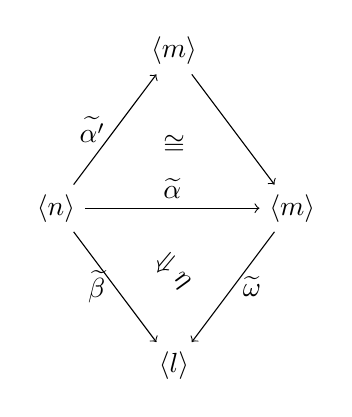
\begin{tikzpicture}
                % Define node positions
                \node (B) at (0, 2) {$\langle n \rangle$}; \node (C) at (3, 2)
                {$\langle m \rangle$}; \node (D) at (1.5, 4) {$\langle m
                \rangle$}; \node (A) at (1.5, 0) {$\langle l \rangle$};
                
                % Draw arrows
                \draw[->] (B) -- (C) node[midway, above] {$\widetilde{\alpha}$};
                \draw[->] (B) -- (A) node[midway, left] {$\widetilde{\beta}$};
                \draw[->] (C) -- (A) node[midway, right] {$\widetilde{\omega}$};
                \draw[->] (B) -- (D) node[midway, left] {$\widetilde{\alpha'}$};
                \draw[->] (D) -- (C) node[midway, right] {$\id$};
                
                % Natural transformation arrow
                \node[rotate=-40] at (1.5, 1.2) {$\Downarrow \eta$}; \node at
                (1.5, 2.8) {$\cong$};
                % \node at (1.7, 1.2) {$\eta$};
            \end{tikzpicture}
        \end{center}
        where $\widetilde{\alpha'}$ is $\alpha' = \alpha$ on finite pointed sets
        but equipped with the trivial collection of configurations
        $\{\id^{\alpha_j}\}_{j \in J}$. Hence, we gain $\widetilde{\omega}_k$ as
        an $\beta^{-1}(k)$-labeled configuration. This diagram in $\Br$:
        \begin{center}
            \begin{tikzpicture}
                % Define node positions
                \node (B) at (0, 2) {$(\omega \circ \alpha)^{-1}(k)$}; \node (C)
                at (3, 2) {$\beta^{-1}(k)$}; \node (A) at (1.5, 0) {$\{k\}$};
                
                % Draw arrows
                \draw[->] (B) -- (C) node[midway, above] {\small $\id$};
                \draw[->] (B) -- (A) node[midway, left] {\small
                $\widetilde{\omega}_k$}; \draw[->] (C) -- (A) node[midway,
                right] {\small $\widetilde{\beta}_k$};
                
                % Natural transformation arrow
                \node at (1.5, 1.2) {$\overset{\eta^{-1}}{\Leftarrow}$};
                % \node[rotate=-40] at (1.5, 1.2) {$\Downarrow \eta$};
            \end{tikzpicture}
        \end{center}
        gives a corresponding composition map in $\B$:
        $$
            \gamma \colon \prod_{p \in {\beta^{-1}(k)}} \Mul_{\B}^{\id^{(p)}}\left(\{X_{p}\}, X_{p}\right)\times \Mul_{\B}^{\widetilde{\beta}_k}\left(\{X_p\}_{p\in \beta^{-1}(k)}, Y_k\right) \to \Mul_{\B}^{\widetilde{\omega}_k} \left(\{X_{i_q}\}_{q \in \omega^{-1}(k)}, Y_k\right).
        $$
        We choose
        \[
            \bar{f}_k \coloneqq \gamma((\id_{X_p})_{p \in {\beta^{-1}(k)}}, g_k).
        \]
        Note, applying the composition, of almost the same diagram but for
        $\eta$, to $\bar{f}_k$ we obtain $g_k$. This follows from the unitality
        property in $\B$ and is precisely why $\bar{f}_k$ can not be chosen
        differently. Hence, $\bar{f}$ is unique. 
        
        Furthermore, with this property the morphism $\widetilde{\alpha}$
        induces a functor of fibers
        \[
            \Bx_{\langle n \rangle} \to \Bx_{\langle m \rangle}
        \]
        sending
        \[
            [X_1, \dots, X_n] \mapsto [Y_1, \dots, Y_m]
        \]
        where $[Y_1, \dots, Y_m]$ corresponds to a cocartesian morphism $f
        \colon [X_1, \dots, X_n] \to [Y_1, \dots, Y_m]$ in $\Bx$. For a
        different choice of cocartesian morphism $h \colon [X_1, \dots, X_n] \to
        [\bar{Y}_1, \dots, \bar{Y}_m]$ we obtain, due to the cocartesian
        property, two unique lifts $\bar{f}, \bar{h}$ that must be inverse to
        one another:
        \begin{center}
            \begin{tikzcd}
                {[X_1, \dots, X_n]} \arrow[rd, "h"'] \arrow[r, "f"] & { [Y_1,
                \dots, Y_m]} \arrow[d, "\bar{h}", dashed, shift left] &
                \rightarrow & \langle n \rangle \arrow[r, "\widetilde{\alpha}"]
                \arrow[rd, "\widetilde{\alpha}"'] & \langle m \rangle
                \\
                                                                    & {
                                                                    [\bar{Y}_1,
                                                                    \dots,
                                                                    \bar{Y}_m]}
                                                                    \arrow[u,
                                                                    "\bar{f}",
                                                                    dashed,
                                                                    shift left]
                                                                    & & &
                                                                    \langle m
                                                                    \rangle
                                                                    \arrow[u,
                                                                    "\id"']
            \end{tikzcd}
        \end{center}
        Hence, the functor is well-defined on objects up to unique isomorphism.
        For morphisms we define:
        \[
            (g \colon [X_1, \dots, X_n] \to [X_1', \dots, X_n'])  \mapsto (\bar{f} \colon [Y_1, \dots, Y_m] \to [Y_1', \dots, Y_m'])
        \]
        where $\bar{f}$ is the unique lift to the cartesian morphism $f$,
        corresponding to the following diagrams:
        \begin{center}
            \begin{tikzcd}
                {[X_1, \dots, X_n]} \arrow[r, "f!"] \arrow[d, "g"'] & {[Y_1,
                \dots, Y_m]} \arrow[d, "\bar{f}", dashed] & {} \arrow[r, "\pi",
                shift right=9] & {} & \langle n \rangle \arrow[d, "\id"]
                \arrow[r, "\widetilde{\alpha}"] & \langle m \rangle \arrow[d,
                "\id"] \\
                {[X_1', \dots, X_n']} \arrow[r, "f'!"]              & {[Y_1',
                \dots, Y_m']}                            & &    & \langle n
                \rangle \arrow[r, "\widetilde{\alpha}"]                  &
                \langle m \rangle                 
            \end{tikzcd}
        \end{center}


        The composition of two morphisms 
        \[
        g \colon [X_1, \dots, X_n] \to [X_1',
        \dots, X_n'], \; g \colon [X_1', \dots, X_n'] \to [X_1'', \dots, X_n'']
        \]
        is being respected as the composition of the unique lifts $\bar{f}$ and
        $\bar{f}'$ lift the diagram and therefore have to be the unique lift for
        $g' \circ g$ and $f$:
        \begin{center}
            \begin{tikzcd}
                {[X_1, \dots, X_n]} \arrow[r, "!f"] \arrow[d, "g"']     & {[Y_1,
                \dots, Y_m]} \arrow[d, "\bar{f}", dashed] \\
                {[X_1', \dots, X_n']} \arrow[r, "!f'"] \arrow[d, "g'"'] &
                {[Y_1', \dots, Y_m']} \arrow[d, "\bar{f}'", dashed]      \\
                {[X_1'', \dots, X_n'']} \arrow[r, "!f''"']              &
                {[Y_1'', \dots, Y_m'']}                         
            \end{tikzcd}
        \end{center}
        \item \todo{write down}
        % \item For $n \in \N$, $1 \leq i \leq n$, the inert morphism
        % \[
        %     \rho^i \langle n \rangle \to \langle 1 \rangle,
        % \]
        % as defined in \ref{eg:rho_i}, induces a functor on fiber categories:
        % \[
        %     P^i \colon \Bx_{\langle n \rangle} \to \Bx_{\langle 1 \rangle}.
        % \]
        % Thus,
        % \[
        %     \prod_{1 \leq i \leq n} P^i \colon \Bx_{\langle n \rangle} \to \left(\Bx_{\langle 1 \rangle}\right)^n
        % \]
        % is fully faithful and essentially surjective. This follows immediately
        % when considering the construction of $P^i$.
        \item By construction of $\Bx$ the following holds: For $X_1, \dots,
        X_n$ colors in $\B$ the morphism
        \[
            \phi \colon [X_1, \dots, X_n] \to [X_i]
        \]
        with $\rho^i$ and $\phi_i = \id_{X_i}$ covers $\rho^i$ for all $1 \leq i
        \leq n$.
    \end{enumerate}
\end{proof}



In the last step, we want to sketch a reconstruction of a colored braided operad
for the following statement:

\begin{prop}
    Let
    \[
        \pi \colon \D \to \Brx
    \]
    be a functor fulfilling the following conditions:
    \begin{enumerate}
    \item For every inert morphism $\alpha \colon \langle n \rangle \to \langle
    m \rangle$ in $\Brx$ and object $X \in \Bx$ there exists a $\pi$-cocartesian
    morphism $f \colon X \to X'$ lifting $\alpha$. In particular, $\alpha$
    induces a functor:
    $$\pi_{\alpha} \colon \Bx_{\langle n \rangle} \to \Bx_{\langle m \rangle}.$$

    \item Let $X \in \Bx_{\langle n \rangle}$ and $X' \in \Bx_{\langle m
    \rangle}$ be objects, $\alpha : \langle n \rangle \to \langle m \rangle$ be
    a morphism in $\Brx$ and let $\Hom_{\Bx}^{\alpha}(X, X')$ be the isomorphism
    class of morphisms which lie over $\alpha$. 
    
    Choose $\pi$-cocartesian morphisms $X' \to X'_i$ lying over the inert
    morphism $\rho^i \colon \langle n \rangle \to \langle 1 \rangle$ for $1 \leq
    i \leq n$. Then the induced map
    \[
        \Hom_{\Bx}^{\alpha}(X, X') \to \prod_{1 \leq i \leq n} \Hom_{\Bx}^{\rho^i \circ \alpha}(X, X_i')
    \]
    is an equivalence of groupoids. 
    
    \item For every finite collection of objects $X_1, \dots, X_n \in
    \Bx_{\langle 1 \rangle}$, there exists an object $X \in \Bx_{\langle n
    \rangle}$ and a collection of $\pi$-cocartesian morphism $X \to X_i$
    covering $\rho^i \colon \langle n \rangle \to \langle 1 \rangle$.
    % \item For all $n \in \N$, there is an equivalence of categories
    % \[
    %     \Bx_{\langle n \rangle} \cong \left(\Bx_{\langle 1 \rangle}\right)^n
    % \]
    % induced by the morphism $\rho^i$ from Example \ref{eg:rho_i}.
    \end{enumerate}
    Then we can reconstruct a colored braided operad $\B$ from $\D$ such that,
    $\D \cong \Bx$ and the functor
    \[
        \Bx \cong \D \overset{\pi}{\to} \Brx
    \]
    is the usual forgetful functor from $\Bx$ to $\Brx$.
\end{prop}

\begin{proof}
    \todo{fix proof since bijection is now missing}
    Let
    \[
        \pi \colon \D \to \Brx
    \]
    be a functor fulfilling the conditions from the statement. We will define a
    colored braided operad $\B$ from $\D$ and $\pi$. The fiber category
    $\D_{\langle 1 \rangle}$ is the underlying category of $\B$. The objects in
    $\D_{\langle 1 \rangle}$ are the colors of $\B$. Let $I$ be a finite set,
    $\widetilde{I} \in \E_2(n)$ an $I$-labeled configuration, $\{X_i\}_{i \in
    I}$ a collection of colors and $Y$ a color. For $\widetilde{I}$ we have a
    bijection $\iota \colon \langle n \rangle^{\circ} \to I$. Using this
    bijection there is an object 
    $$\left(X_{\iota(i)}\right)_{1 \leq i \leq n} \in \left(\Bx_{\langle 1
    \rangle}\right)^n$$ corresponding to some object $X$ in $\D_{\langle n
    \rangle}$ by the equivalence in condition (2). Then, 
    \[
        \Mul_{\B}^{\widetilde{I}}\left(\{X_i\}_{i \in I}, Y\right)
    \]
    is the set of morphisms $f \colon X \to Y$ in $\D$ such that $\pi(f)$
    corresponds to the active morphism
    \[
        \langle n \rangle \to \langle 1 \rangle
    \]
    with configuration $\widetilde{I}$ in $\Brx$.

    The composition map is induced by the composition map in $\D$.
    \todo{elaborate on this if time} 
    The identity morphisms in $\B$ are given by the identity morphisms in the
    fiber category $\D_{\langle 1 \rangle}$, i.e., for each color $X \in
    \D_{\langle 1 \rangle}$, the identity morphism $\id_X$ in $\D$ defines the
    identity morphism in $\Mul_{\B}^{\id}(\{X\}, X)$. The associativity
    requirement is met as the composition if defined via the composition map in
    $\D$ which is associative. The unitality condition is also induced by the
    unitality in $\D$.
    \todo{equivalence}
\end{proof}